\documentclass{beamer}
\usetheme{Boadilla}
\usepackage{hyperref}
\usepackage{graphicx}
\usepackage{fancyvrb}
\usepackage{multicol}
\usepackage{subfig}
\usepackage[
    backend=biber, 
    natbib=true,
    style=numeric,
    sorting=none,
    style=verbose-ibid,
    labelyear
]{biblatex}
\addbibresource{citations.bib}
\usepackage{pgfpages}
\usepackage{xcolor}
\definecolor{ao(english)}{rgb}{0.0, 0.5, 0.0}
\definecolor{burgundy}{rgb}{0.5, 0.0, 0.13}
\setbeameroption{show notes}
\setbeameroption{show notes on second screen=right}

\title{Neural audio synthesis}
\subtitle{WaveNet, SampleRNN, and the waveform domain}
\author{Sevag Hanssian}
\institute{McGill University}
\setbeamertemplate{navigation symbols}{}

\begin{document}

\begin{frame}
\maketitle
\href{run:./funkybass.wav}{SOUND CHECK}
\end{frame}

\begin{frame}
	\frametitle{Physical sound waves}
	\begin{figure}
	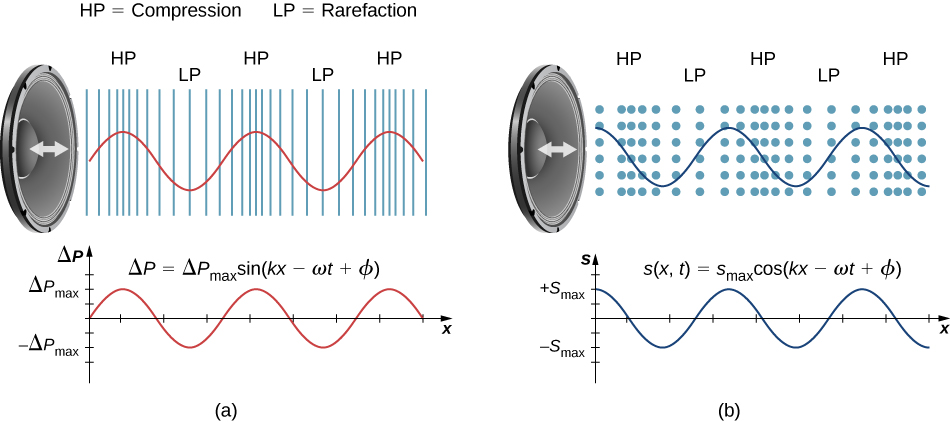
\includegraphics[height=5cm]{./1_sound_pressure.jpg}
		\caption{a) air pressure vs. distance, b) air molecule displacement \footfullcite{airpressure}}
	\end{figure}
\end{frame}

\note{
\begin{itemize}
	\item
		Sound waves can be modelled by air pressure variations or air molecule displacement
\end{itemize}
}

\begin{frame}
	\frametitle{Waveforms (human pov)}
	\begin{figure}
		\subfloat[Tonotopic organization of the inner ear\footfullcite{tonotopic}]{{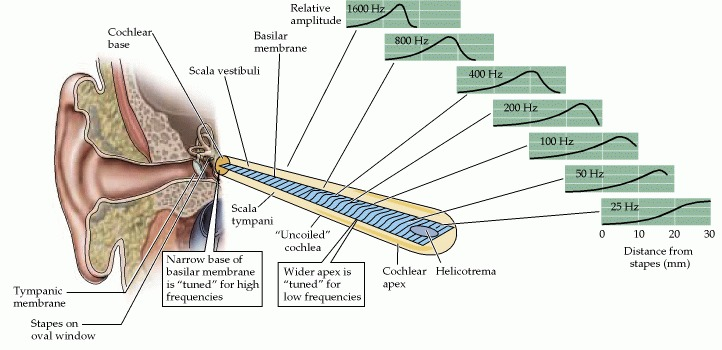
\includegraphics[width=6.5cm]{./1_5_tonotopic.jpg} }}
		\hspace{0.2em}
		\subfloat[Ascending auditory pathways \footfullcite{auditorypathway}]{{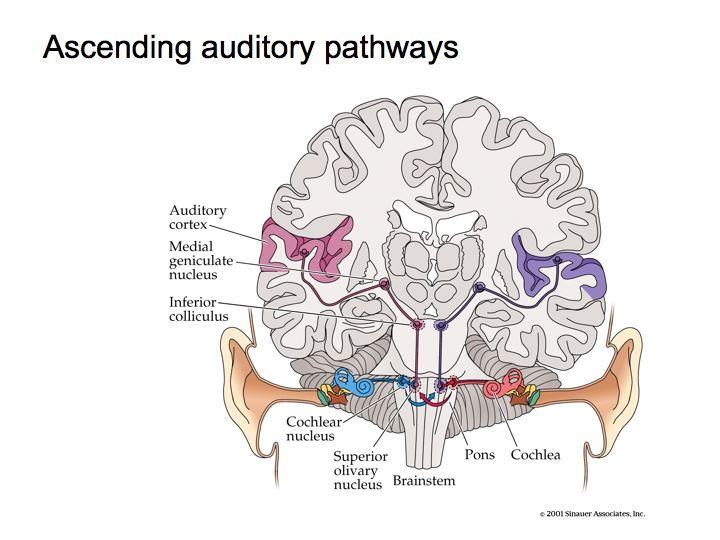
\includegraphics[width=5cm]{./1_7_auditory_pathway.jpg} }}
		\caption{Human auditory neural network}
	\end{figure}
\end{frame}

\note{
\begin{itemize}
	\item
		Hearing is when our ears detect sound pressure variations
	\item
		Vibrates our basilar membrane by frequency component
	\item
		Travels up the auditory nerve for further processing (so we can recognize and enjoy speech, music, etc.)
	\item
		An actual ``neural network''
\end{itemize}
}

\begin{frame}
	\frametitle{Waveforms (digital pov)}
	\begin{figure}
		\subfloat[Microphone/transducer\footfullcite{shuremic}]{{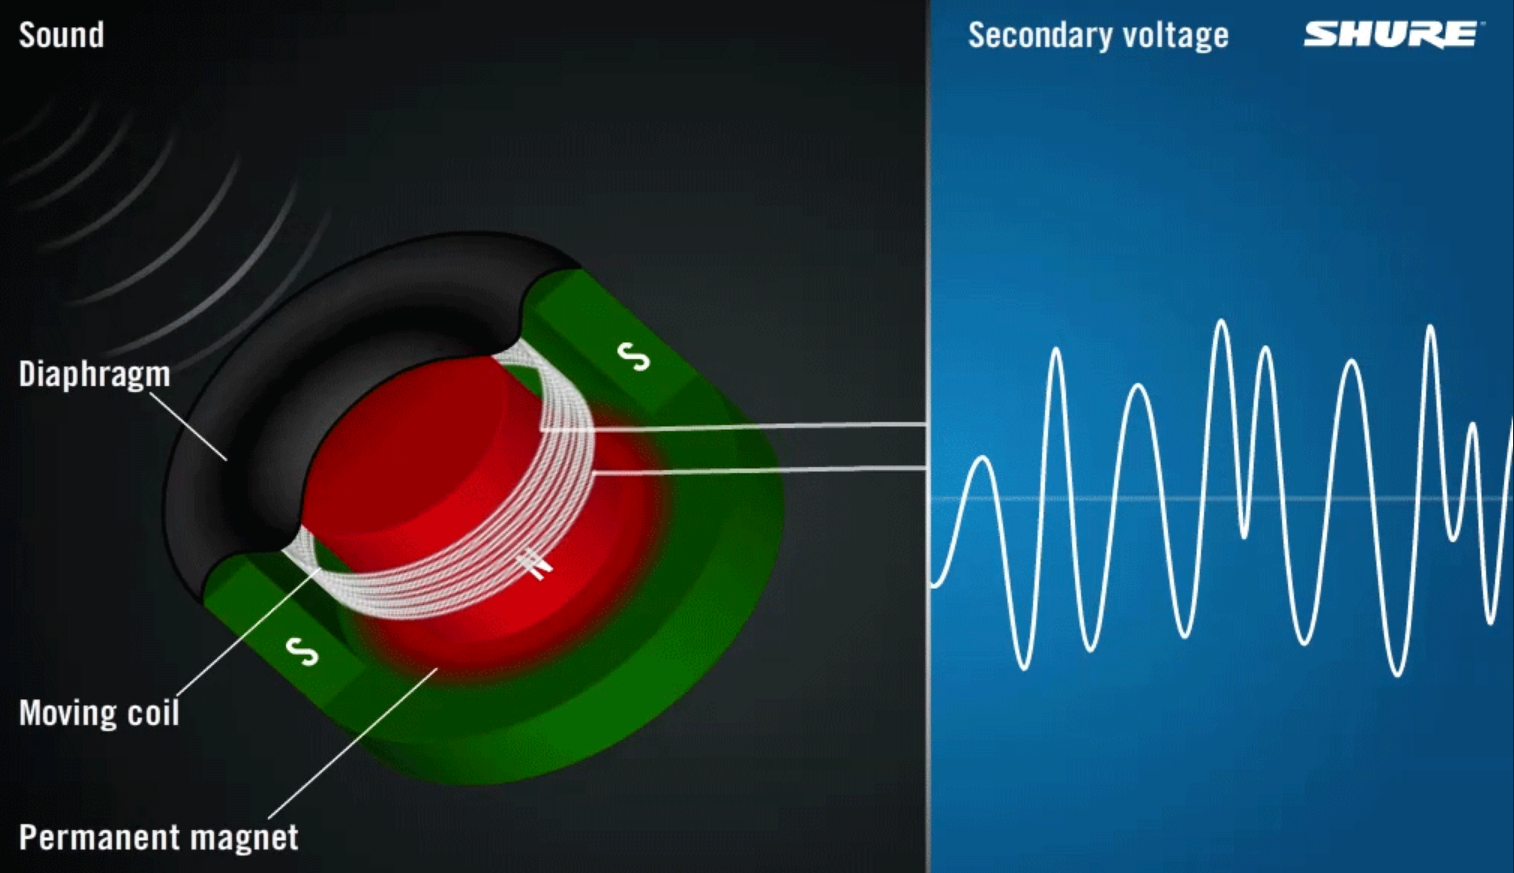
\includegraphics[height=3.5cm]{./2_transducer.png} }}
		\hspace{0.2em}
		\subfloat[Analog to digital\footfullcite{l2p}]{{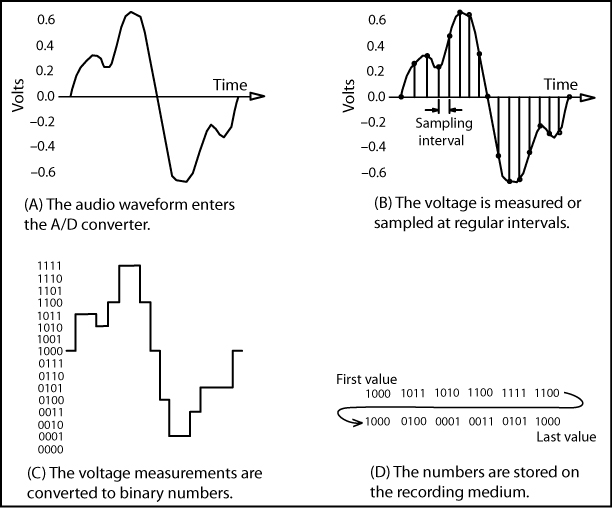
\includegraphics[height=3.5cm]{./3_adc_quantize.jpg} }}
		\caption{Sound pressure wave to analog signal to digital signal}
	\end{figure}
\end{frame}

\note{
\begin{itemize}
	\item
		Microphones are transducers -- convert sound pressure variations into an analog electric signal
	\item
		Analog signals are continuous in both time and range of values, so it must be sampled and quantized (pulse code modulation), Nyquist-Shannon sampling theorem -- the fundamental bridge between continuous-time and discrete time
	\item
		Process is done in reverse for taking this digital signal and outputting it through speakers/headphones
	\item
		Wave to waveform
\end{itemize}
}

\begin{frame}[fragile]
	\frametitle{Waveform domain}
	\begin{figure}
	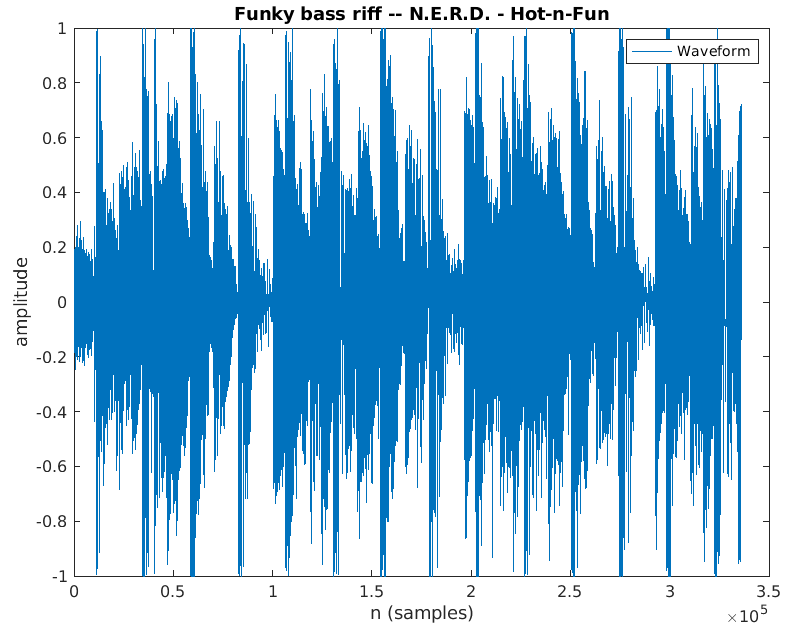
\includegraphics[height=4.5cm]{./4_funkybass.png}
		\caption{Bass riff waveform \href{run:./funkybass.wav}{(CLICK2PLAY)} \footfullcite{hotnfun}}
	\end{figure}
	\vspace{-1em}
	How meaningful is it?\\
	{\small{\Verb#>> disp(x(50:128)); 0.0609, 0.0456, 0.0326, 0.0375, ...#}}
\end{frame}

\begin{frame}
	\frametitle{Frequency domain}
	\vspace{-1em}
	\begin{figure}
	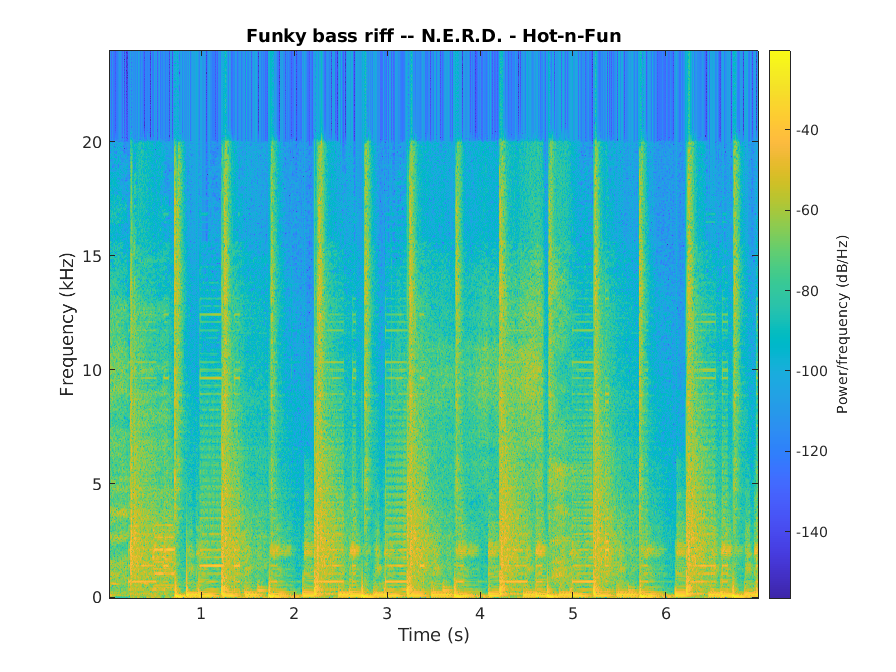
\includegraphics[height=4cm]{./5_funkybass_spectrogram.png}
	\end{figure}
	\vspace{-1em}
	\textbf{\textcolor{red}{Cons}}
	Often in the spectral domain, phase information is omitted\footfullcite{phase}, sacrificing timbre quality in the recreation (\href{run:./original_phase.wav}{good} vs. \href{run:./random_phase.wav}{bad})\\
	\textbf{\textcolor{ao(english)}{Pros}}
	Dimensionality of recognizeable audio features (notes, melodies, utterances) is more compact \footfullcite{samplernn}
\end{frame}

\note{
	\begin{itemize}
		\item
			We discard the phase component when analyzing audio, because it is not informative for most of the things we could be interested in. phase is very important because it meaningfully affects our perception \textbf{when generating sound}. phase hard because
			\begin{itemize}
			\item
				it is an angle between 0 and 2pi and wraps around (princarg)
			\item
				it becomes effectively random as the magnitude tends towards 0, because noise starts to dominate;
			\item
				absolute phase is less meaningful, but relative phase differences over time matter perceptually.
			\end{itemize}
		\item
			Counterpoint is that modeling the waveform domain implicitly preserves phase information, perceptually important
		\item
			Counterpoint is that the waveform needs hundres of thousands of samples for simple audio features -- from the sampleRNN paper, one of the primary methods i'll be introducing today
	\end{itemize}
}

\begin{frame}[fragile]
	\frametitle{Symbolic domain}
	The highest human level of representation for musical structure\\
	e.g. bass tab \footfullcite{ultimateguitar}
	\begin{small}
		\begin{verbatim}
		G|--------------------------|
		D|------3--3--4-----3--4----|
		A|----3--3--------3---------|
		E|--------------------------|
		\end{verbatim}
	\end{small}
	\begin{quote}
	Automatic music generation dates back to more than half a century. A prominent approach is to generate music symbolically in the form of a piano roll, which specifies the timing, pitch, velocity, and instrument of each note to be played. This has led to impressive results like producing Bach chorals, polyphonic music with multiple instruments, as well as minute long musical pieces.\\
	But symbolic generators have limitations -- they cannot capture human voices or many of the more subtle timbres, dynamics, and expressivity that are essential to music.\footfullcite{jukebox1}
	\end{quote}
\end{frame}

\note{
	\begin{itemize}
		\item
			Algorithmic music composition -- MUMT 306 material
		\item
			I'm not even aware of how many of these exist. Tabs, sheet music, etc.
	\end{itemize}
}

\begin{frame}
	\frametitle{Interlude: machine learning in acoustics}
	\begin{figure}
	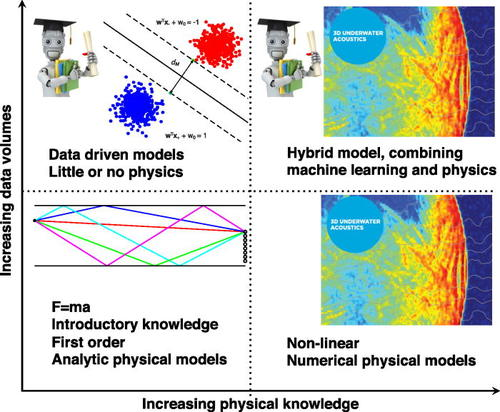
\includegraphics[height=4cm]{./6_5_ml_acoustics.jpg}
		\caption{Analytic physical models (lower left) give basic insights about physical systems. More sophisticated models, reliant on computational methods (lower right), can model more complex phenomena. Whereas physical models are reliant on rules, which are updated by physical evidence (data), ML is purely data-driven (upper left). By augmenting ML methods with physical models to obtain hybrid models (upper right), a synergy of the strengths of physical intuition and data-driven insights can be obtained \footfullcite{mlacoustics}}
	\end{figure}
\end{frame}

\note{
	\begin{itemize}
		\item
			First two papers i'll discuss, purely neural audio synthesis, are from the top left. Unstructured, whacky, figure out what you can from the provided audio
		\item
			Lastly I'll mention an alternative approach, top right -- mixing our known acoustical physical models with machine learning and deep learning to train on real audio and discover optimal parameters
	\end{itemize}
}

\begin{frame}
	\frametitle{Sound synthesis -- wavetables and sinusoidal oscillators}
	Wavetable synthesis is perhaps the oldest technique for creating sounds with computers. It involves \textbf{the storage of a single period of a periodic waveform} in a circular buffer. By varying the ``speed'' with which a read pointer is advanced through the buffer, one can achieve output waveforms of different frequencies \footfullcite{3071}.\\\ \\
	Sound synthesis algorithms are typically described and implemented using primitive signal processing ``building blocks'' called \textbf{unit generators}. Create complex synthesis by combining multiple oscillators (see next page) \footfullcite{3072}, \footfullcite{3073}, \footfullcite{3074}.
\end{frame}

\note{
	307 material -- sound synthesis
	\begin{itemize}
		\item
			Can simulate more complex sound with multiple wavetables, envelopes, unit generators, oscillators.
		\item
			So, the computer is not \textit{creating} a new waveform -- it's modifying one already supplied to create outputs with different frequencies.
		\item
			Similarly, sine wave generators generate a simple basic waveform on which operations are applied and combined to create complex sounds
		\item
			Or using FFT synthesis (summation of sines)
		\item
			We're either using an existing waveform or combining simple waveforms, through frequency domain principles, to generate complex waveforms
	\end{itemize}
}

\begin{frame}
\frametitle{Sound synthesis -- sinusoidal oscillators}
	\begin{figure}
		\subfloat{{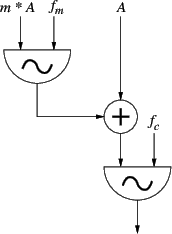
\includegraphics[height=4cm]{./6_am.png} }}
		\hspace{0.2em}
		\subfloat{{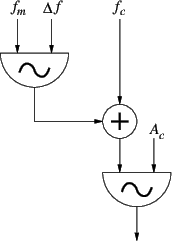
\includegraphics[height=4cm]{./6_fm.png} }}
		\hspace{0.2em}
		\subfloat{{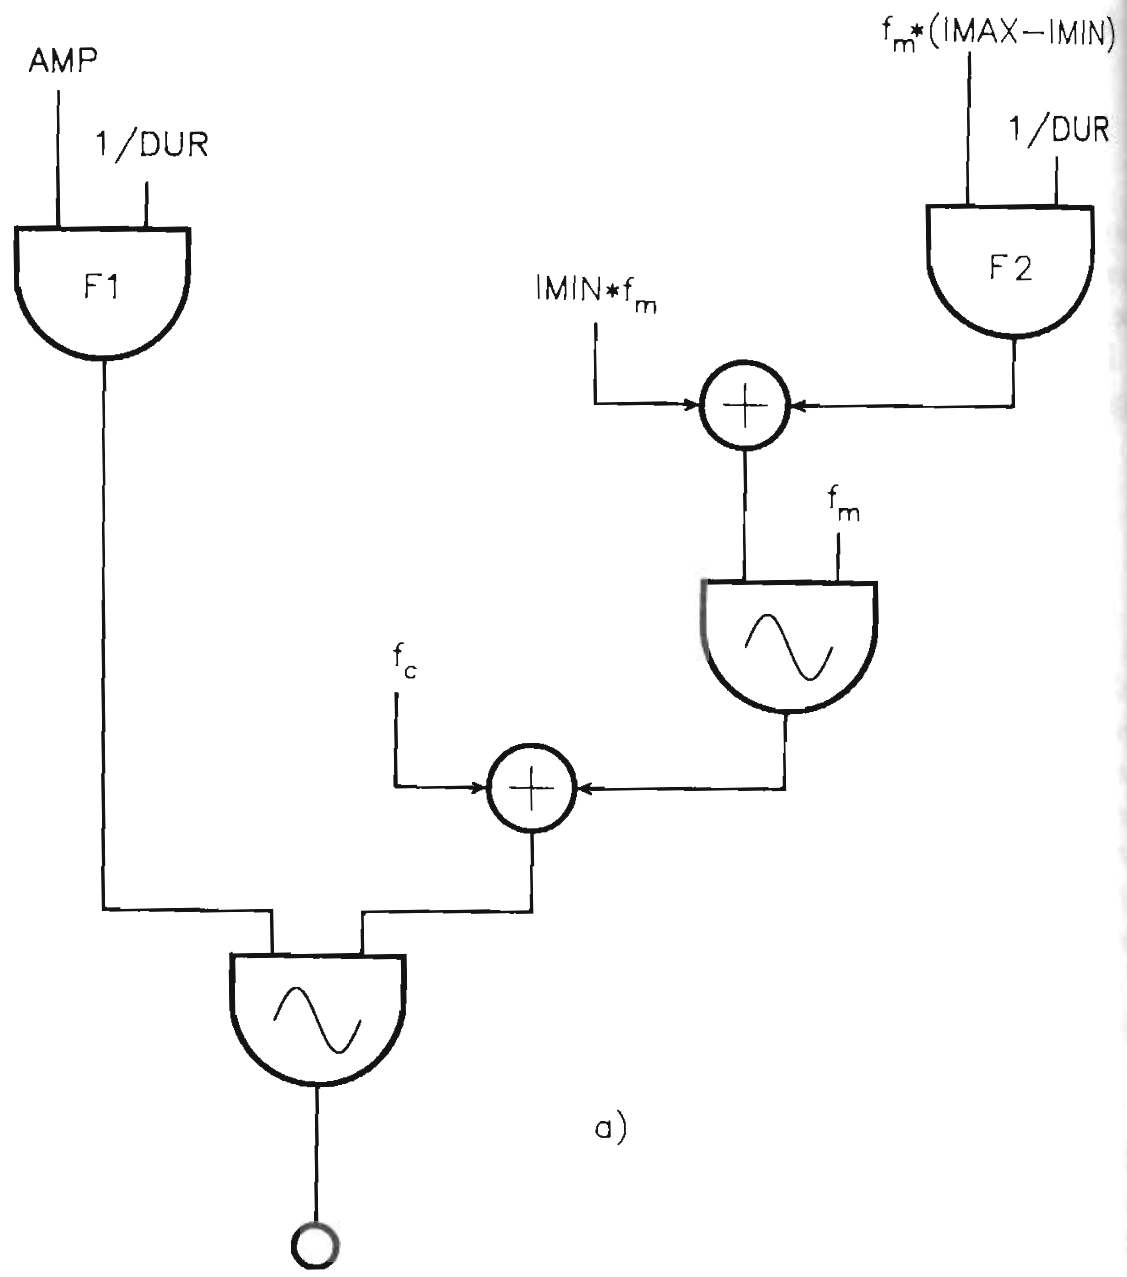
\includegraphics[height=5cm]{./6_chowning_fm_clarinet.png} }}
		\caption{Sinusoidal oscillators in AM synthesis, FM synthesis, Chowning clarinet model (citations on previous slide)}
	\end{figure}
\end{frame}

\note{
\begin{quote}
	 In 1967, Chowning realized that complex sounds could be generated using only two oscillators when the output of one oscillator is connected to the frequency input of a second oscillator. Essentially, the first oscillator generates a pure tone that modulates the frequency of the second oscillator in a way that produces a complex tone, like a string vibrating.
\end{quote}
}

\begin{frame}
	\frametitle{Neural audio synthesis}
	\begin{quote}
		The question of generating musical signals has been extensively studied over the past decades. Most of the previous approaches on this topic were \textbf{defined in the spectral domain as a complex set of relatively simple manipulation (subtractive, additive or modulation synthesis)}. However, several recent breakthroughs in audio waveform generative models based on neural networks (Oord, 2016 \textbf{WaveNet}) have obtained astounding results in speech synthesis both qualitatively and quantitatively (Mehri, 2016 \textbf{SampleRNN}). These systems rely on learning the structure of audio waveforms directly from a given set of audio files, without computing a spectral transform and in an unsupervised manner.\footfullcite{intro1}
	\end{quote}
\end{frame}

\note{
	\begin{itemize}
		\item
			In traditional synthesis we create complex waveforms by combining simple ones
		\item
			In 2018, we have the computational power and models to make sense of the waveform directly
	\end{itemize}
}

\begin{frame}
	\frametitle{WaveNet}
	Concatenative TTS: database of short speech fragments recombined to form complete utterances\\\ \\

	Parameteric TTS: information to generate data is stored as model parameters, contents and characteristics of speech are controlled via model inputs. Parametric models generate audio through vocoders -- sound less natural than concatenative\\\ \\

	WaveNet changes this paradigm by directly modelling the raw waveform of the audio signal, one sample at a time. As well as yielding more natural-sounding speech, using raw waveforms means that WaveNet can model any kind of audio, including music. \footfullcite{wavenet}, \footfullcite{wavenetpaper}
\end{frame}

\note{
	\begin{itemize}
		\item
			Introduced by DeepMind London (Google) in September 2016.
		\item
			Derives from PixelCNN -- similarity with audio, large arrays of numbers with patterns
		\item
			TTS = text-to-speech
		\item
			 difficult to modify the voice (for example switching to a different speaker, or altering the emphasis or emotion of their speech) without recording a whole new database
	\end{itemize}
}

\begin{frame}
	\frametitle{Artificial neural networks}
	\begin{figure}
	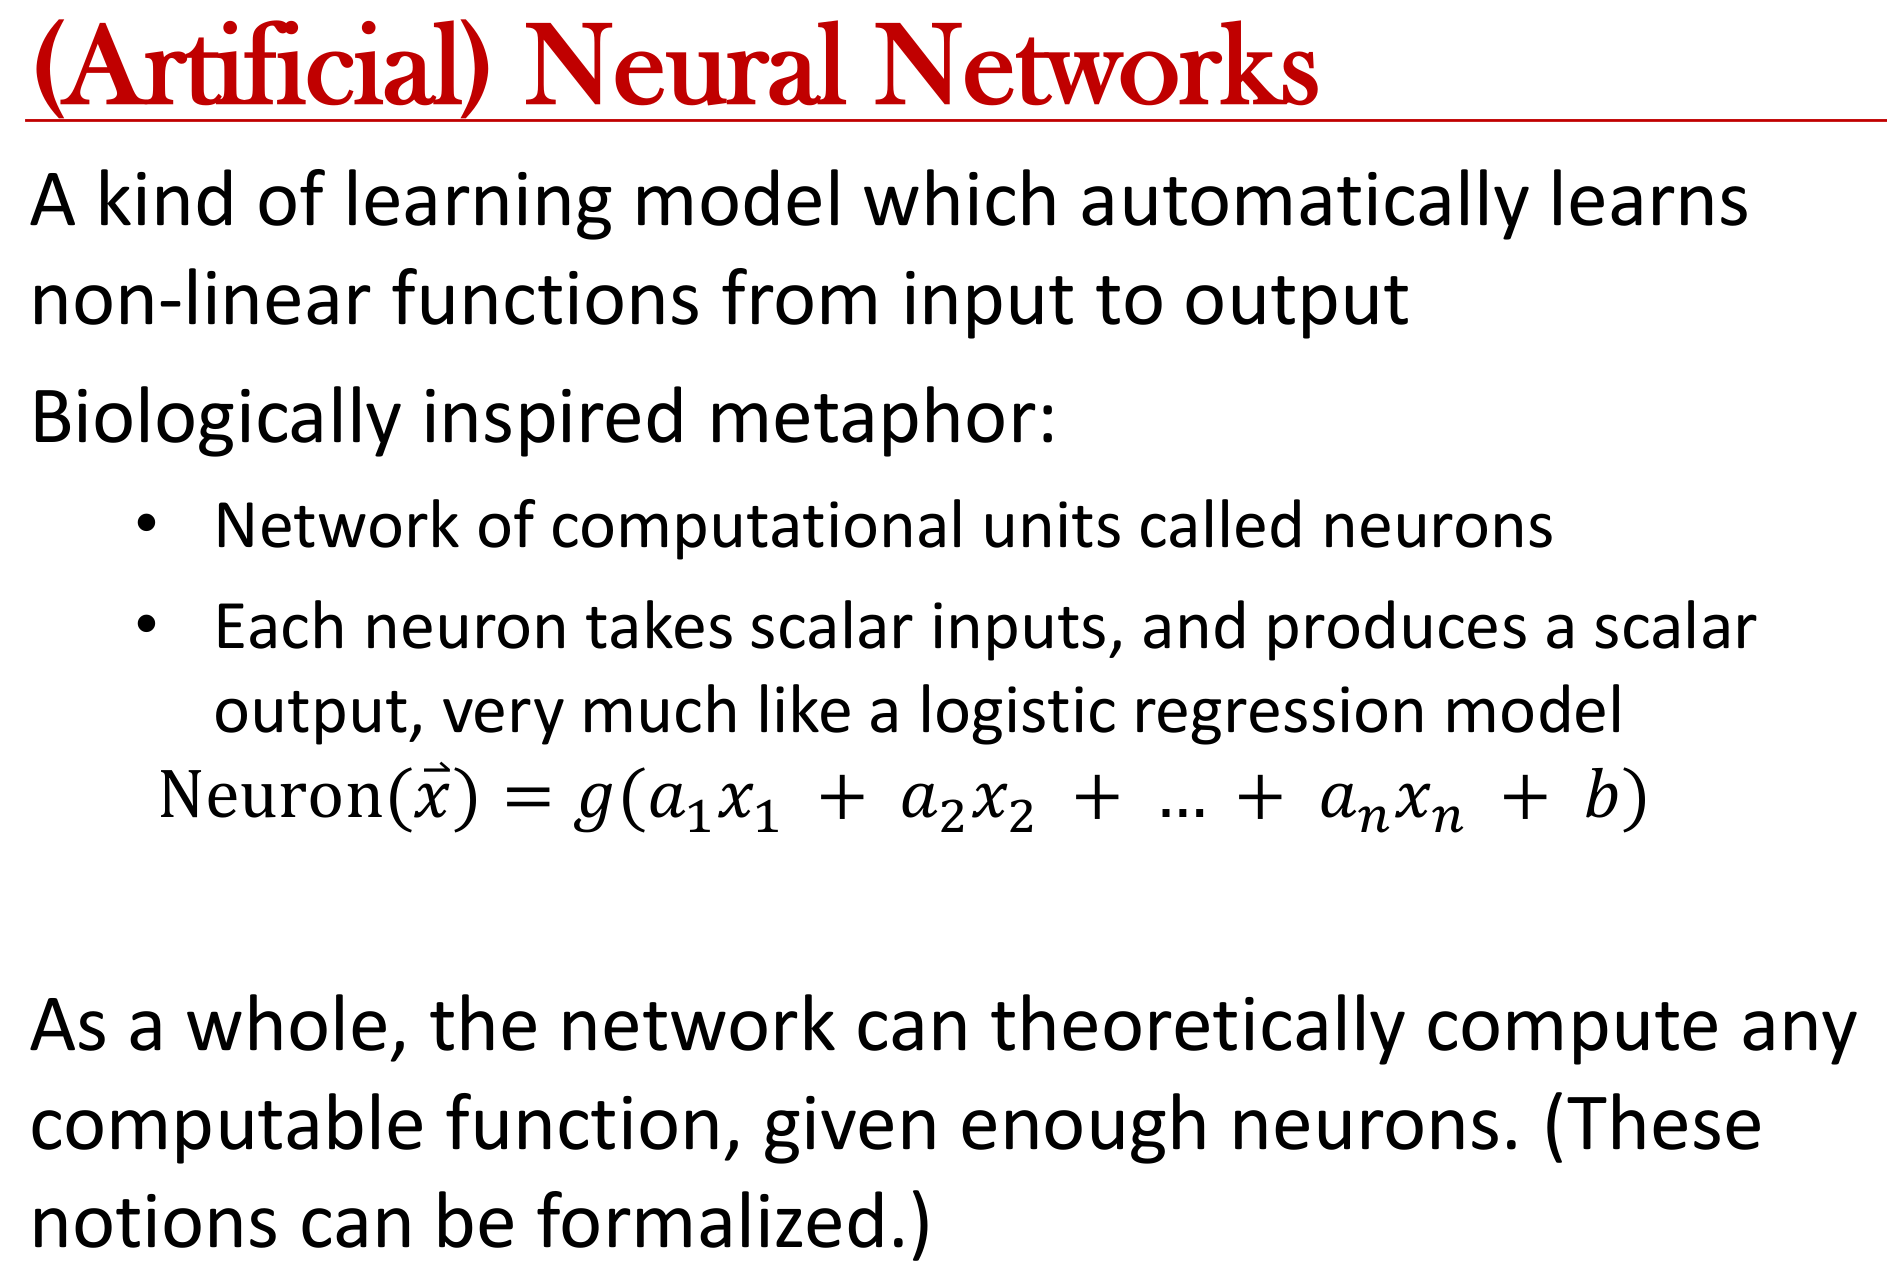
\includegraphics[width=10cm]{./nn_intro.png}
		\caption{Artificial neural network primer \footfullcite{comp5501}}
	\end{figure}
\end{frame}

\note{
	\begin{itemize}
		\item
			I can't tell you its meaningful, but my brain certainly knows it.
		\item
			Psychoacoustics -- after the inputs to the system (basilar membrane etc.) are activated, the end result is that sound creates a bunch of firing neurons that travel ``up the 
		\item
			Unsupervised learning -- you only had to listen to music to figure out patterns. Nobody had to tell you what patterns to look for
		\item
			Contrast to FEM -- did a very light bit of research, not enough...
	\end{itemize}
}

\begin{frame}
	\frametitle{WaveNet -- details}
	\begin{itemize}
		\item
			Causality -- y[n] can only depend on \{x[n], x[n-1], ...\}
		\item
			Autoregressive -- audio samples are generated by estimating likely next values based on past values
		\item
			Convolutions -- this is the same convolution from DSP\footfullcite{fftconv}
		\item
			Dilated convolutions -- widen the time scale of learning by increasing space between samples
		\item
			$\mu$-law quantization: quantization mapping to critical bands, a common speech technique\footfullcite{mulaw}
	\end{itemize}
\end{frame}

\note{
	\begin{itemize}
		\item
			makes sense for audio which moves forward in time
		\item
			Convolution and correlation are related. The goal is to find repeating strong patterns in waveform data by doing convolutions somewhere in the neural network's hidden layers
		\item
			Mu-law isnt used in sampleRNN, only wavenet
	\end{itemize}
}

\begin{frame}
	\frametitle{WaveNet diagram}
	\begin{figure}
	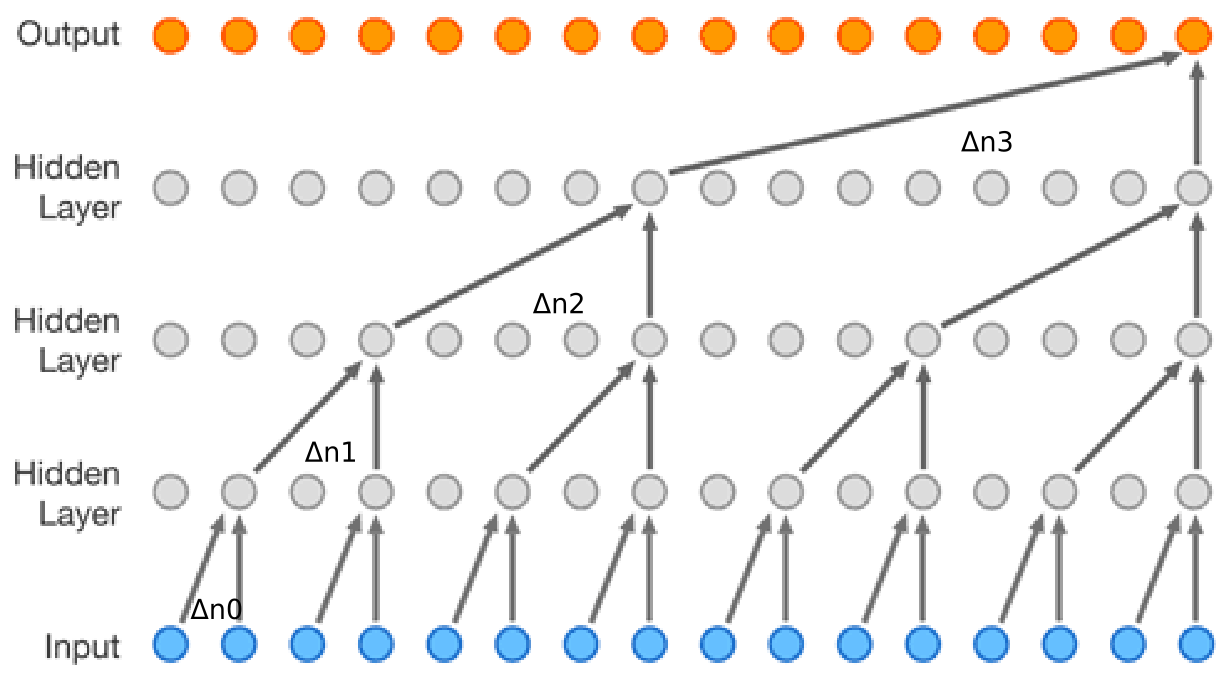
\includegraphics[height=5cm]{./7_wavenet_annot.png}
		\caption{How wavenet computes samples of output y[n] from historical samples \{x[n], x[n-1], ...\}}
	\end{figure}
\end{frame}

\note{
	\begin{itemize}
		\item
			Same diagram as wavenet, i added the delta t annotations
		\item
			delta t0 = 1 sample timescale (patterns in 1/fs = dT)
		\item
			delta t1 = 2 sample timescale, etc.
	\end{itemize}
}

\begin{frame}
	\frametitle{WaveNet math}
	\begin{figure}
	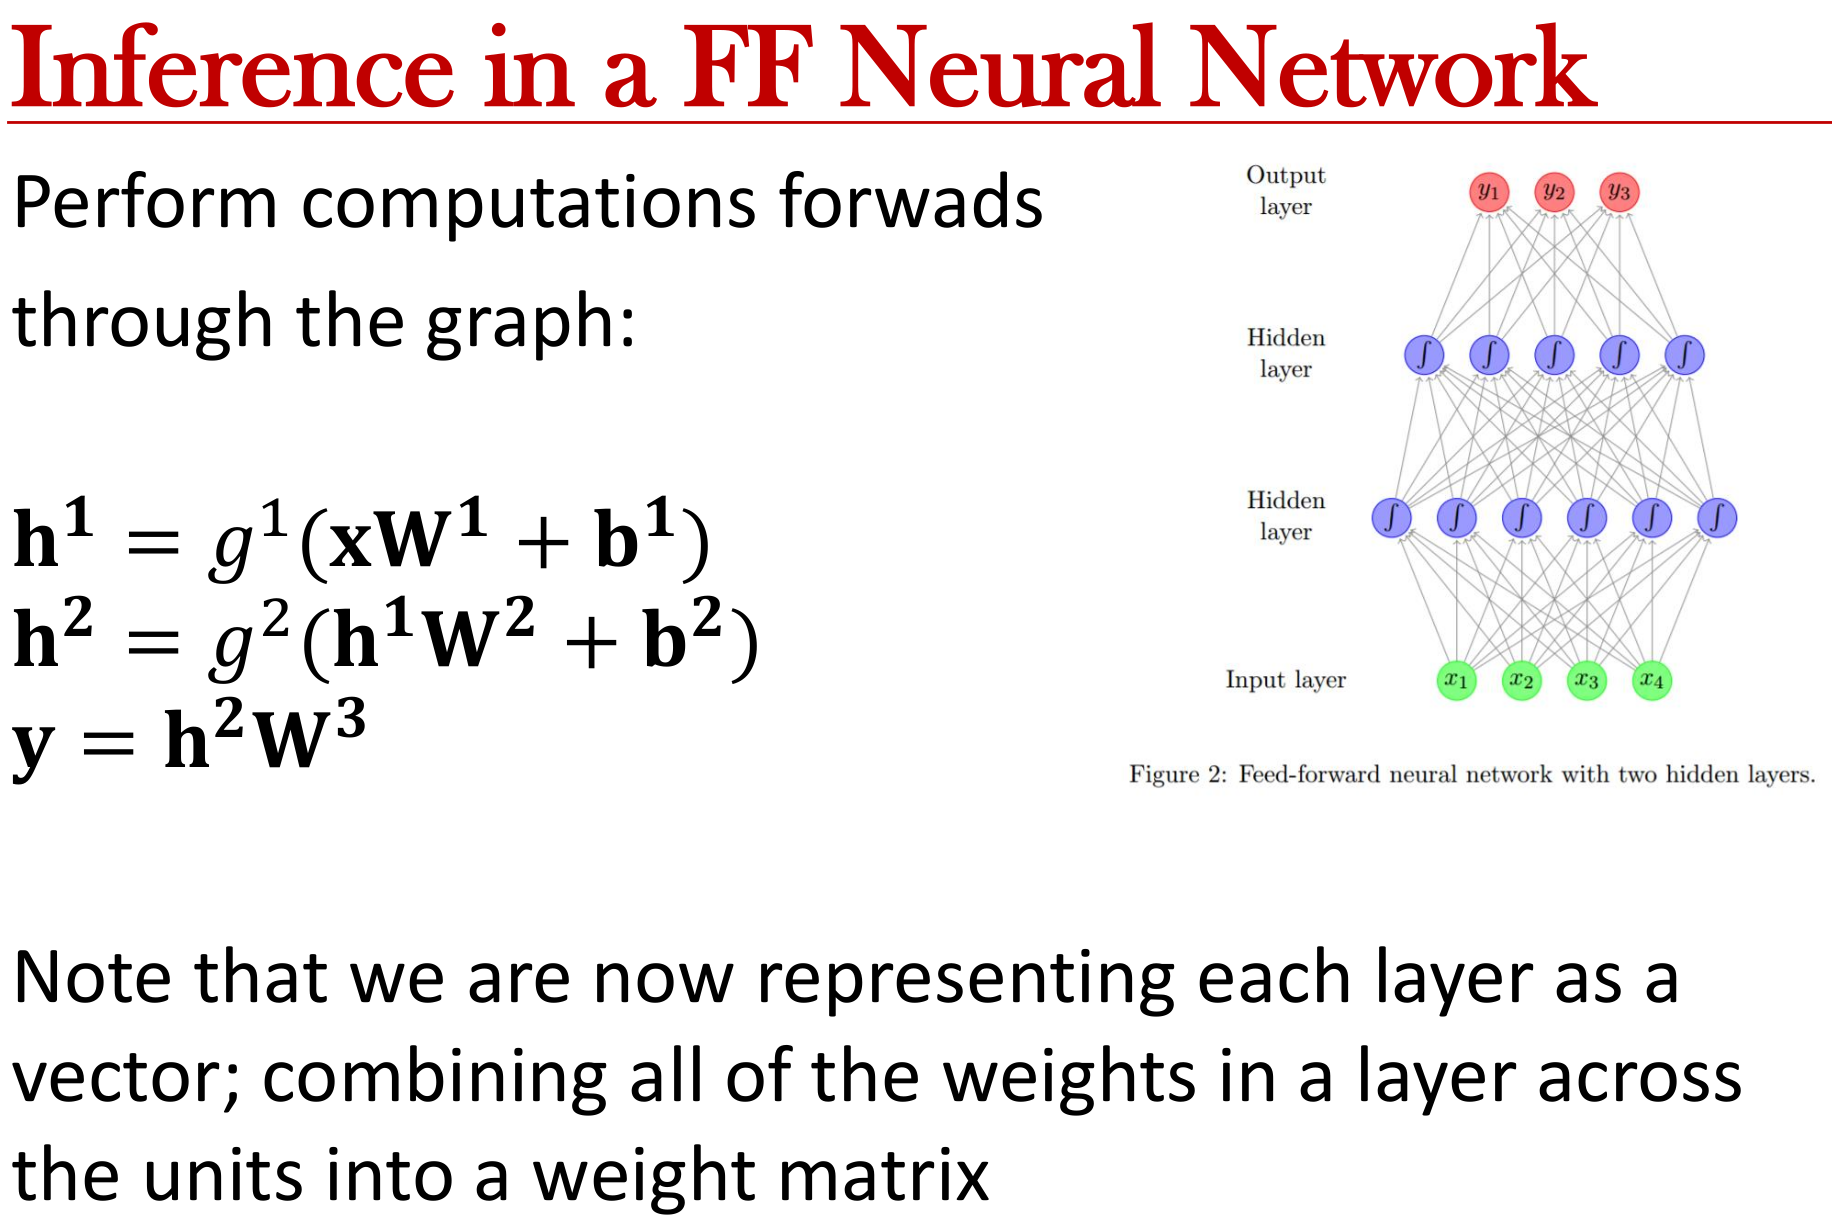
\includegraphics[width=10cm]{./nn_inference.png}
		\caption{Example of how the previous diagram maps to some equations \footfullcite{comp5502}}
	\end{figure}
\end{frame}

\begin{frame}
	\frametitle{WaveNet examples}
	All examples are from WaveNet blog post\footfullcite{wavenet}
	\begin{itemize}
		\item
			Unconditioned speech (i.e. let the machine do whatever it wants): \href{run:./wavenet_speech_unconditional.wav}{CLICK TO PLAY}
		\item
			Conditioned speech, English (i.e. train machine to learn a specific phrase*): \href{run:./wavenet_speech_conditioned_english.wav}{CLICK TO PLAY}
		\item
			Conditioned speech, Mandarin: \href{run:./wavenet_speech_conditioned_mandarin.wav}{CLICK TO PLAY}
		\item
			Unconditional music**: \href{run:./wavenet_sample_1.wav}{CLICK TO PLAY}
		\item
			Unconditional music: \href{run:./wavenet_sample_2.wav}{CLICK TO PLAY}
	\end{itemize}\ \\
	\vspace{1em}
	*: it's unclear to me how -- the paper has precious few details\\
	**: they provide no examples of conditioned (i.e. structured) music
\end{frame}

\begin{frame}
	\frametitle{SampleRNN}
	Use RNNs to learn long-term patterns:\\
	\begin{quote}
		raw audio signals are challenging to model because they contain structure at very different scales: correlations exist between neighboring samples as well as between ones thousands of samples apart. SampleRNN helps to address this challenge by using a hierarchy of modules, each operating at a different temporal resolution.\footfullcite{samplernn}
	\end{quote}
	Contrast with WaveNet dilations:
	\begin{quote}
		In order to deal with long-range temporal dependencies needed for raw audio generation, we develop new architectures based on dilated causal convolutions\footfullcite{wavenet}
	\end{quote}
\end{frame}

\begin{frame}
	\frametitle{What's an RNN}
	Recurrent neural networks:
	\begin{quote}
		Recurrent neural networks, also known as RNNs, are a class of neural networks that allow previous outputs to be used as inputs while having hidden states.\footfullcite{rnn}
	\end{quote}\\
	So, it generates samples at a micro-temporal scale (like WaveNet) for realistic timbre/notes, and then the generated samples feed back into the network which has also learned macro-temporal patterns (e.g. how notes follow other notes), to generate audio which exhibits patterns at multiple temporal scales.\\
\end{frame}

\note{
	\begin{itemize}
		\item
			 Different scales of patterns -- that's music exactly
		 \item
			 The main insight behind SampleRNN is that audio in particular exhibits salient patterns at multiple timescales, and that these patterns and features are composed hierarchically. For example, timbre is shaped by patterns over very short timescales, while musical events and gestures like bowing or striking an instrument happen over longer timescales. Melodies are composed of a series of musical events, which are often grouped into compositional structures like bars or phrases, which are further grouped into sections and then full songs. (Karl Hiner)
	\end{itemize}
}

\begin{frame}
	\frametitle{SampleRNN diagram}
	Note how similar it is to WaveNet. WaveNet ``dilates'' the convolutions to go from a small time step to a large one  -- SampleRNN ``upsamples'' the vector to bump up the temporal resolution
	\begin{figure}
	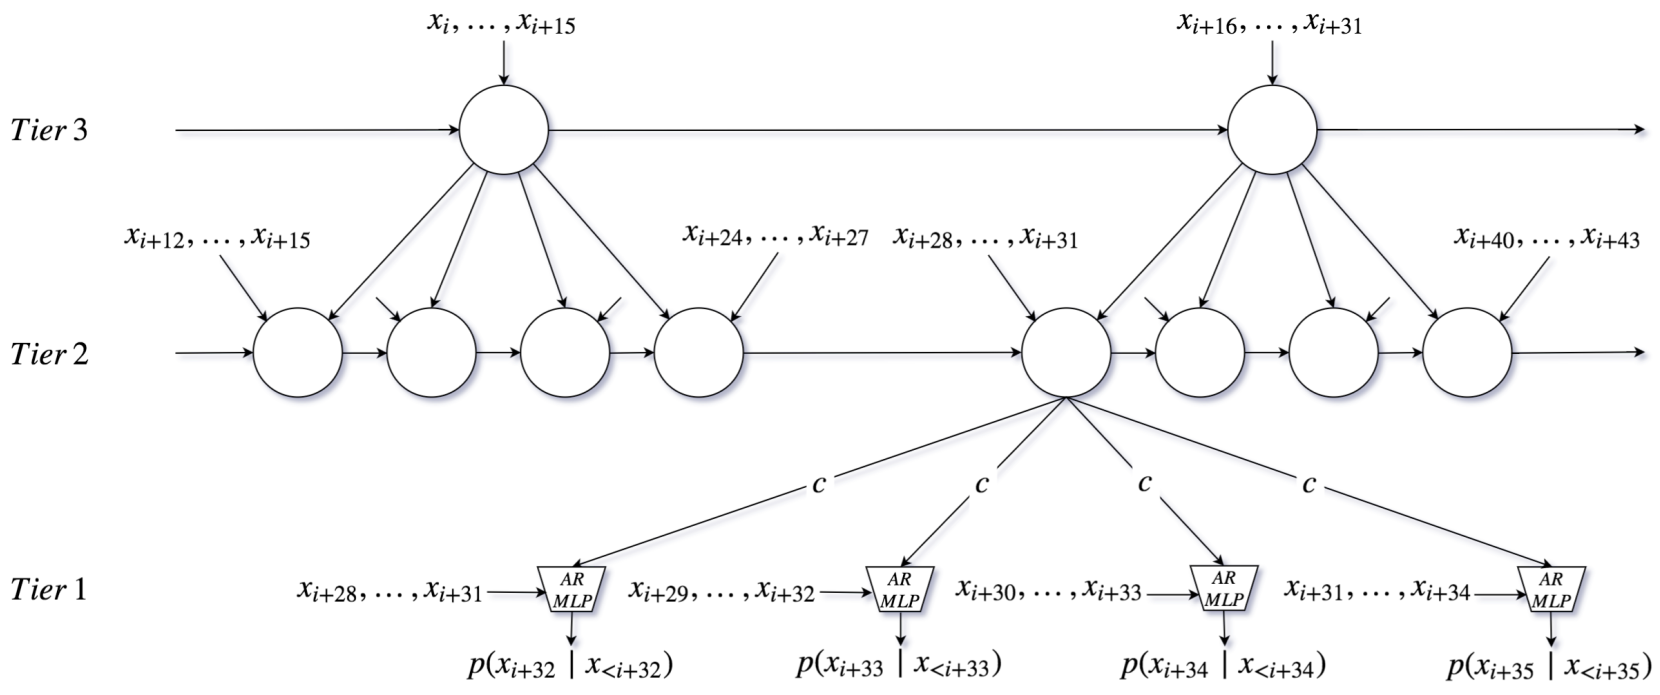
\includegraphics[height=5cm]{./8_samplernn.png}
		\caption{How SampleRNN computes samples of output y[n] from historical samples \{x[n], x[n-1], ...\}}
	\end{figure}
\end{frame}

\note{
	\begin{itemize}
		\item
			For me, dilation (spreading out the input signal) is the same as upsampling (spreading out the input signal)
		\item
			Notice how the diagram shows the broad similarity in their architecture
	\end{itemize}
}

\begin{frame}
	\frametitle{SampleRNN in practise}
	So what does SampleRNN actually look like? Up-to-date implementation, PRiSM SampleRNN based on Tensorflow 2\footfullcite{prism1}, \footfullcite{prism2}. Your best bet at getting up and running (works for me).
	\begin{itemize}
		\item
			Own an NVIDIA GPU + modern Linux to set up Python dependencies
		\item
			Gather training data (wav files), run train.py and generate.py (README has example commands and description of parameters)
		\item
			How to choose parameters?
			\begin{quote}
				Training neural networks is, ironically, more of an art than a science, and depends on a lot of trial and error... So I'd say just dive into it with the default settings initially, and then see what results you get.\footfullcite{prism3}
			\end{quote}
	\end{itemize}
\end{frame}

\note{
	\begin{itemize}
		\item
			Science vs. art?
		\item
			What's the line between science, art, and magic?
		\item
			Is it art if I have no clue what's going on?
	\end{itemize}
}

\begin{frame}
	\frametitle{SampleRNN examples}
	Examples are from independent blog post\footfullcite{samplernnsamples}*
	\begin{itemize}
		\item
			Unconditioned piano music: \href{run:./samplernn_sample_2.mp3}{CLICK TO PLAY}
		\item
			Unconditioned music, Dawn of Midi: \href{run:./samplernn_sample_1.mp3}{CLICK TO PLAY}
		\item
			Unconditioned music, Animals as Leaders**: \href{run:./aamgen_epoch_45.wav}{CLICK TO PLAY}
		\item
			Unconditioned music, Animals as Leaders: \href{run:./aamgen_epoch_75.wav}{CLICK TO PLAY}
		\item
			Unconditioned music, Animals as Leaders: \href{run:./aamgen_epoch_80.wav}{CLICK TO PLAY}
	\end{itemize}\ \\
	\vspace{1em}
	*: Karl Hiner mentions that he never got results as good as WaveNet 's public releases. Purports that they do lots of specialized training\\
	**: from my own experiments of running PRiSM SampleRNN\footfullcite{prism2}
\end{frame}

\note{
	\begin{itemize}
		\item
			The non-reproduceability problem personified?
		\item
			Hidden trade secrets?
	\end{itemize}
}

\begin{frame}
	\frametitle{Traits of WaveNet and SampleRNN}
	Referring to WaveNet generated speech quality:
	\begin{quote}
		Unconditional generation from this model manifests as ``babbling'' due to the lack of longer term structure\footfullcite{wavenetcrit1}
	\end{quote}\\\ \\
	Referring to WaveNet and SampleRNN listening experiments trained on classical and techno music:
	\begin{quote}
		we first compare the related audio file sets of both experiments. After listening to the music samples, we conclude that none of the four sets contain audio that even slightly resembles music. The files generally sound noisy and random.\footfullcite{wavenetcrit2}
	\end{quote}
\end{frame}

\note{
	\begin{itemize}
		\item
			WaveNet and SampleRNN are good at learning on a micro-temporal level (up to individual instrument onsets, notes, timbres). Needs further conditioning to enforce longer-term structure (melody, song structure, etc.)
		\item
			Incoherent medium/longer-term structure:
		\item
			In that first paper, they start discussing ways of training WaveNet by enforcing longer-term structure
	\end{itemize}
}

\begin{frame}
	\frametitle{Unstructured can be good}
	The dadabots\footfullcite{dadabots1} use the incoherence of SampleRNN to their advantage\\
	Who are they? ``We make raw audio neural networks that can imitate bands''. Example: \href{https://www.youtube.com/watch?v=MwtVkPKx3RA}{Relentless Doppleganger}\\\ \\
	\begin{quote}
		[...] we want the output to overfit short timescale patterns (timbres, instruments, singers, percussion) and underfit long timescale patterns (rhythms, riffs, sections, transitions, compositions) so that it sounds like a recording of the original musicians playing new musical compositions in their style.\footfullcite{dadabots2}
	\end{quote}
\end{frame}

\note{
	This is my project idea. It'll be heavier on the literature -- I'll need to deep dive to understand the innards of the machine learning/neural networks, but it's too soon to do a significant contribution or novel work -- I'm new to machine learning. I want to create a fake artist with fake music using one or many machine learning-based approaches.
}

\begin{frame}
	\frametitle{Towards structure}
	Jukebox\footfullcite{jukebox1}, \footfullcite{jukebox2} addresses the long input problem with an autoencoder that compresses raw audio to a lower-dimensional space by discarding perceptually irrelevant information. Then trains a model to generate audio in this compressed space, and upsample back to the raw audio space.\\
	\vspace{0.5em}
	Tacotron 2\footfullcite{tacotron21}, \footfullcite{tacotron22} uses an 80-dimensional audio spectrogram with frames computed every 12.5 milliseconds to capture not only pronunciation of words, but also various subtleties of human speech, including volume, speed and intonation. These features are converted to a waveform using a WaveNet-like architecture.
\end{frame}

\note{
	\begin{itemize}
		\item
			Note the 2 ways of dealing with wavenet shortcomings
		\item
			Jukebox relies on operating on a compressed version of the waveform, so it can become computationally feasible to learn longer-term (minutes) musical structure. Opens itself up to suffering from imperfect recreation - e.g. Griffin-Lim phase reconstruction
		\item
			Tactron 2 combines spectral features for long-term structure (utterances, words) and wavenet for the synthesis to the waveform. Best of both worlds
	\end{itemize}
}

\begin{frame}
	\frametitle{Recall}
	\begin{figure}
	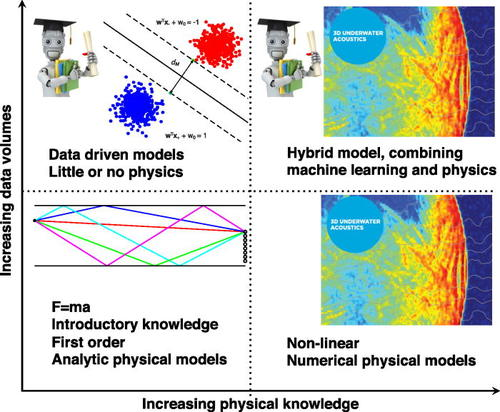
\includegraphics[height=4cm]{./6_5_ml_acoustics.jpg}
		\caption{By augmenting ML methods with physical models to obtain hybrid models (upper right), a synergy of the strengths of physical intuition and data-driven insights can be obtained \footfullcite{mlacoustics}}
	\end{figure}
\end{frame}

\begin{frame}
\frametitle{Middle ground}
% double column pros cons like thanos presentation with colors
	\textbf{\textcolor{burgundy}{Traditional synthesis}}: structured building blocks based on frequency and/or symbolic representation. Fiddly parameters, imperfect recreations\\
	\textbf{\textcolor{burgundy}{Fully neural audio synthesis}}: realistic timbre, dynamics, delays, ``human'' traits, create natural sounds. Unstructured black box\\
	\textbf{\textcolor{ao(english)}{Differentiable DSP}}\footfullcite{ddsp1}, \footfullcite{ddsp2}
	\begin{quote}
		a collection of linear filters and sinusoidal oscillators can create the sound of a realistic violin if the frequencies and responses are tuned in just the right way. However, it is difficult to dynamically control all of these parameters by hand, which is why synthesizers with simple controls often sound unnatural and ``synthetic''.

		With DDSP, we use a neural network to convert a user's input into complex DSP controls that can produce more realistic signals.
	\end{quote}
\end{frame}

\note{
	\begin{itemize}
		\item
			Learn complex parameters to traditional DSP building blocks, rather than throwing out the baby with the bathwater.
	\end{itemize}
}

\begin{frame}
	\frametitle{Differentiability}
	\begin{quote}
		Derivatives, mostly in the form of gradients and Hessians, are ubiquitous in machine learning. Automatic differentiation (AD), also called algorithmic differentiation or simply ``autodiff'', is a family of techniques similar to but more general than backpropagation for efficiently and accurately evaluating derivatives of numeric functions expressed as computer programs.\footfullcite{differentiable}
	\end{quote}
	The gradient, or slope, of the loss function. How does machine learning know that one set of random parameters is better than another? How does it ``learn'' to improve? By moving in a direction that reduces the slope of error, i.e. gradient descent.
\end{frame}

\note{
	\begin{itemize}
		\item
			Differentiability is not new. Relevant in many forms of numerical computation e.g. fem. Just very generalized in neural networks
		\item
			``Differentiable'' -- machine learning is often done with gradients -- gradient descent. The machine ``learns'' by reducing the error through the gradient. As DSP building blocks are differentiable, they can thus be machine learned (or more accurately, parameters can be estimated, and from the differentiability, the resulting quality improvement can be measured e.g. compared to a real violin sound).
	\end{itemize}
}

\begin{frame}
	\frametitle{Conclusions}
	\begin{itemize}
		\item
			Modeling audio in the waveform domain is now feasible with the computational power of modern machines and neural networks
		\item
			WaveNet and SampleRNN were the trendsetters, and there is a lot of derivative work since then (WaveRNN, Jukebox, etc.)
		\item
			Advantages include learning realistic timbre, dynamics, intonations, etc. directly from the waveform. No reconstruction problems
		\item
			Disadvantages include unstructured/unreliable outputs, black box (difficult to understand) computational model
	\end{itemize}
\end{frame}

\note{
	\begin{itemize}
		\item
			It's taken me 3 weeks of training so far to get even really bad outputs. Computational power is a real limitation
		\item
			We can't compete with BigCos and their own special sauce (computation, storage, in-house expertise)
	\end{itemize}
}

\end{document}
